%
% Hello! Here's how this works:
%
% You edit the source code here on the left, and the preview on the
% right shows you the result within a few seconds.
%
% Bookmark this page and share the URL with your co-authors. They can
% edit at the same time!
%
% You can upload figures, bibliographies, custom classes and
% styles using the files menu.
%
% If you're new to LaTeX, the wikibook at
% http://en.wikibooks.org/wiki/LaTeX
% is a great place to start, and there are some examples in this
% document, too.
%
% Enjoy!
%
\documentclass[12pt,a4paper]{article}

\usepackage[german]{babel}
\usepackage[utf8x]{inputenc}
\usepackage{amsmath}
\usepackage{enumitem}
\usepackage{graphicx}
\usepackage{fancyhdr}
\usepackage{longtable}
\usepackage{lastpage}
\usepackage[bottom]{footmisc}
\usepackage{listings}
\usepackage{rotating}
\usepackage{changepage}   % for the adjustwidth environment
\usepackage[cm]{fullpage}
\usepackage[parfill]{parskip}
\usepackage[table]{xcolor}

\title{Entwicklerdokumentation Mikroprogrammierung}
\author{Amar Saljic, Arseniy Vershinin, Jonathan Kienzle}
\date{12. Juli 2013}

\pagestyle{fancy}
\fancyhead{} % clear all header fields
\fancyhead[RE,LO]{\emph{Entwicklerdokumentation Mikroprogrammierung - Gruppe 50}}
\renewcommand{\headrulewidth}{0pt} % no line in header area
\fancyfoot{} % clear all footer fields
\fancyfoot[LE,RO]{\thepage /\pageref{LastPage}}           % page number in "outer" position of footer line
%\fancyfoot[RE,LO]{\emph{Entwicklerdokumentation Mikroprogrammierung - Gruppe 50}} % other info in "inner" position of footer line

\begin{document}
\definecolor{lightgray}{gray}{0.9}
\maketitle

\thispagestyle{fancy}

\section{Übersicht}

Das Programm \emph{strlen}, welches die Länge einer Zeichenkette in Zeichen ermittelt, wurde auf zwei Arten implementiert:
\begin{enumerate}
\item Als Maschinenprogramm
\item Als spezieller Maschinenbefehl in einem gesonderten Mikroprogramm
\end{enumerate}
Die zu zählende Zeichenkette liegt im Unicode-Format (16 bit pro Zeichen) im Hauptspeicher und das abschließende Nullzeichen (0x0000) wird nicht mitgezählt.

\section{Implementierung}

\subsection{Allgemeines}
Die Funktionsweise beider Implementierungen kann mittels Pseudocode folgendermaßen veranschaulicht werden:
	

\begin{lstlisting}
length(startAddress) {
    currentAddress = startAddress
    
    characterAtAddress(currentAddress) != 0 {
    	currentAddress = currentAddress + 1
    }
    return currentAddress - startAddress
}
\end{lstlisting}
In den folgenden Abschnitten wird die genaue Implementierung der Programme erläutert. 

Dem Namen jeder Mikroinstruktion wurde jeweils der entsprechend Opcode, welcher vom Dokument \emph{``miziel.ps''} spezifiziert wird, vorangestellt (z.B. 38: mov\_imm\_rb). Die tatsächliche Mikroprogrammspeicheradresse der einzelnen Mikroinstruktionen wird entsprechend der Funktionsweise des MPROM von JMic folgendermaßen berechnet: \(Opcode * 16\). 

Die Standardinstruktion IFETCH steht an der Adresse 0 im Mikroprogrammspeicher und sorgt dafür, dass der nächste Befehl aus dem Hauptspeicher geladen wird und der Befehlszähler inkrementiert wird. Die Implementierung dieses Programms wird im Folgenden nicht beschrieben. 

\subsection{Mikroprogramm}
Das Mikroprogramm besteht aus sechs Mikroinstruktionen, die ab Addresse 0x100 (entspricht dem Opcode 10) im Mikroprogrammspeicher liegen und den folgenden Aufbau haben:

\begin{center}
\rowcolors{1}{lightgray}{white}
\footnotesize
  \begin{tabular}{| p{18cm}|}
  	\hline
    10: strlen\_ra \\
    \hline
    \raisebox{-0.4cm}{
\includegraphics[width=18cm]{strlen_1.png}} \\[0.3cm]
    \hline
    Die Inhalte des Registers \emph{ra} werden nach \emph{r1} kopiert, um die Anfangsadresse der Zeichenkette zu sichern.\\
    \hline
    
    %r1\_addressbus	\\
    %\hline
    \raisebox{-0.4cm}{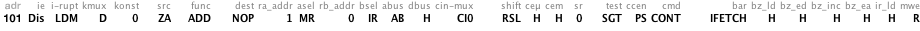
\includegraphics[width=18cm]{strlen_2.png}} \\[0.3cm]
    \hline
    Die in \emph{r1} gespeicherte Adresse wird mithilfe des Y-MUX auf den Addressbus gelegt, wodurch sich die adressierten Daten im nächsten Takt auf dem Datenbus befinden. Mit dieser Instruktion beginnt die Schleifenbedingung aus dem Pseudocode.\\
    \hline
    
    \raisebox{-0.4cm}{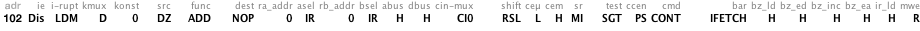
\includegraphics[width=18cm]{strlen_3.png}} \\[0.3cm]
    \hline
    Die Daten, die auf dem Datenbus liegen (\emph{[r1]}), werden mit dem Nullzeichen \emph{0} verglichen, indem sie mit dem Zero-Eingang addiert und die Flags des Mikrostatusregisters entsprechend gesetzt werden.\\
    \hline
    
    %cmp\_zero \\
    %\hline
    \raisebox{-0.4cm}{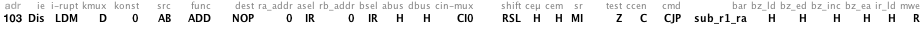
\includegraphics[width=18cm]{strlen_4.png}} \\[0.3cm]
    \hline
    Mithilfe des TEST-Flags wird überprüft, ob durch die vorherige Instruktion der Wert 0 entstanden ist (entspricht der Situation \emph{[r1]} == 0). Falls ja, wird die Schleife beendet und es wird zur letzten Instruktion gesprungen. \\
    \hline
    
    %inc\_r1, jmp\_imm \\
    %\hline
    \raisebox{-0.4cm}{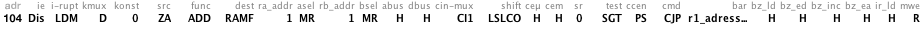
\includegraphics[width=18cm]{strlen_5.png}} \\[0.3cm]
    \hline
   	\emph{r1} wird inkremetiert und es wird zum Anfang der Schleifenbedingung (Instruktionsadresse 101) gesprungen, um das nächste Zeichen zu überprüfen.\\
    \hline
    
    %sub\_r1\_ra \\
    %\hline
    \raisebox{-0.4cm}{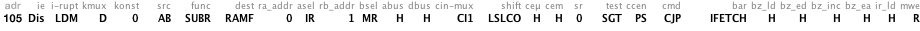
\includegraphics[width=18cm]{strlen_6.png}} \\[0.3cm]
    \hline
   	Es wird \emph{r1} - \emph{r0} berechnet und in \emph{r1} gespeichert. Diese Instruktion wird mit dem Sprung nach IFETCH beendet. Das Ergebnis des Programms befindet sich nun im Register \emph{r1}.\\
    \hline
    
  \end{tabular}
\end{center}

\subsection{Maschinenprogramm}

Das Maschinenprogramm wurde basierend auf den im Dokument \emph{``miziel.ps''} spezifizierten Befehlen implementiert. Das Programm liegt im Hauptspeicher ab Addresse 0x0000 und ist folgendermaßen aufgebaut:

\begin{adjustwidth}{0cm}{}
\begin{center}
  \begin{longtable}{|p{2cm}|p{2cm}|p{2cm}|p{10.7cm}|}
  	\hline
    Addresse & Wert & Mnemo & Kommentar \\
    
    \hline
    0x0000 & 0x3802 & mov 0 r2 & Initialisiere Register \emph{r2} mit dem Wert 0. Dieser Schritt ist für den späteren Aufruf von \emph{cmp} notwendig, da die Zielarchitektur keine \emph{cmp}-Operation spezifiziert, die den direkten Vergleich eines Immidiates mit dem Inhalt einer Speicherzelle ermöglicht. \\
    
    \hline
    0x0001 & 0x0000 & imm = 0 & Wert 0 \\
    
    \hline
    0x0002 & 0x0401 & mov r0 r1 & Kopiere die Anfangsadresse der Zeichenkette, die über \emph{r0} übergeben wurde, nach \emph{r1}. Der Wert dieses Registers entspricht der Addresse des aktuell zu überprüfenden Zeichens. \\
    
    \hline
    0x0003 & 0x3212 & cmp [r1] r2 & Vergleiche das aktuelle Zeichen mit der in \emph{r2} gespeicherten Konstante 0, welche das Ende einer Zeichenkette markiert. Diese Instruktion entspricht der Schleifenbedingung aus dem Pseudocode.\\
    
    \hline
    0x0004 & 0x8100 & jmpz imm & Springe zum Ende des Programms, falls das Ende der Zeichenkette erreicht wurde (die vorherige Instruktion ergab 0 und die Flags wurden entsprechend gesetzt). \\
    
    \hline
    0x0005 & 0x0009 & imm = 9 & Wert 9 \\
    
    \hline 
    0x0006 & 0x4001 & inc r1 & Das Ende der Zeichenkette wurde nicht erreicht. Inkrementiere die Adresse des aktuellen Zeichens. \\
    
    \hline 
    0x0007 & 0xB000 & jmp imm & Springe zur Schleifenbedingung. \\
    
    \hline
    0x0008 & 0x0003 & imm = 3 & Wert 3 \\
    
    \hline
    0x0009 & 0x1401 & sub r0 r1 & Berechne die Länge der Zeichenkette (Substraktion \emph{r1} - \emph{r0}) und speichere sie in Register \emph{r1}. \\
    
    \hline
    
  \end{longtable}
\end{center}
\end{adjustwidth}


Die für die Zielarchitektur spezifizierten Befehle werden in der unten stehenden Tabelle erläutert. Jeder Befehl wird mit einem Sprung zu IFETCH beendet.

\begin{center}
\rowcolors{1}{lightgray}{white}
\footnotesize
  \begin{tabular}{|p{18cm}|}
  	\hline
    38: mov\_imm\_rb \\
    \hline
    \raisebox{-0.4cm}{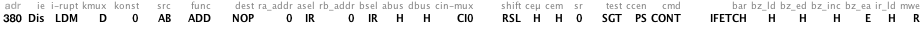
\includegraphics[width=18cm]{mov_imm_1.png}} \\[0.3cm]
    \hline
   Der Inhalt des Befehlszählers wird auf den Addressbus gelegt und das MWE-Flag wird auf R gesetzt.\\

    \hline
    \raisebox{-0.4cm}{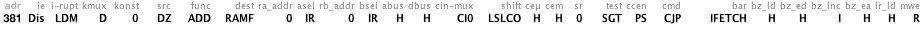
\includegraphics[width=18cm]{mov_imm_2.png}} \\[0.3cm]
    \hline
   Die Daten vom Datenbus werden im Register \emph{ra} gespeichert und der Befehlszähler wird inkrementiert, um den Immidiate-Wert zu überspringen.\\
    \hline
    
  \end{tabular}
\end{center}

\vspace{0.5cm}

\begin{center}
\rowcolors{1}{lightgray}{white}
\footnotesize
  \begin{tabular}{|p{18cm}|}
  	\hline
    04: mov\_ra\_rb \\
    \hline
    \raisebox{-0.4cm}{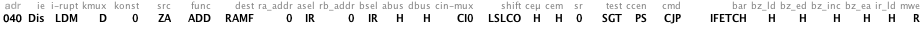
\includegraphics[width=18cm]{mov.png}} \\[0.3cm]
    \hline
   Der Inhalt des Registers \emph{ra} wird mit dem Zero-Eingang addiert und das Ergebnis in \emph{rb} gespeichert.\\
    \hline
  \end{tabular}
\end{center}

\vspace{0.5cm}

\begin{center}
\rowcolors{1}{lightgray}{white}
\footnotesize
  \begin{tabular}{|p{18cm}|}
  	\hline
    40: inc\_rb \\
    \hline
    \raisebox{-0.4cm}{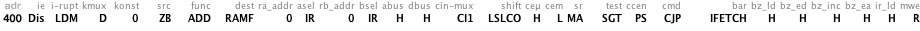
\includegraphics[width=18cm]{inc.png}} \\[0.3cm]
    \hline
   Der Inhalt des Registers \emph{rb} wird mit dem Zero-Eingang und dem Wert 1, der aus dem CIN\_MUX stammt, addiert und das Ergebnis in \emph{rb} gespeichert. Die Maschinenstatusregister-Flags werden dabei entsprechend gesetzt.\\
    \hline
  \end{tabular}
\end{center}

\vspace{0.5cm}

\begin{center}
\rowcolors{1}{lightgray}{white}
\footnotesize
  \begin{tabular}{|p{18cm}|}
  	\hline
    14: sub\_ra\_rb \\
    \hline
    \raisebox{-0.4cm}{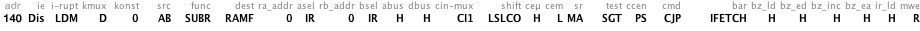
\includegraphics[width=18cm]{sub.png}} \\[0.3cm]
    \hline
   Der Inhalt des Registers \emph{ra} wird vom Inhalt des Registers \emph{rb} substrahiert und das Ergebnis in \emph{rb} gespeichert. Die Maschinenstatusregister-Flags werden dabei entsprechend gesetzt.\\
    \hline
  \end{tabular}
\end{center}

\vspace{0.5cm}

\begin{center}
\rowcolors{1}{lightgray}{white}
\footnotesize
  \begin{tabular}{|p{18cm}|}
  	\hline
    32: cmp\_[ra]\_rb \\
    \hline
    \raisebox{-0.4cm}{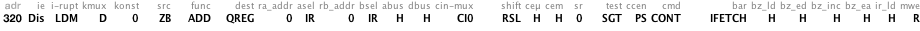
\includegraphics[width=18cm]{cmp_1.png}} \\[0.3cm]
    \hline
   Der Inhlalt des Registers \emph{rb} wird im Register \emph{Q} zwischengespeichert.\\
    \hline
    
    \raisebox{-0.4cm}{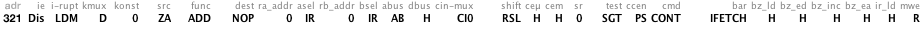
\includegraphics[width=18cm]{cmp_2.png}} \\[0.3cm]
    \hline
   Der Inhalt des Registers \emph{ra} wird auf den Addressbus gelegt und das MWE-Flag auf R gesetzt, um die Daten aus \emph{[ra]} im nächsten Takt lesen zu können.\\
    \hline
    
    \raisebox{-0.4cm}{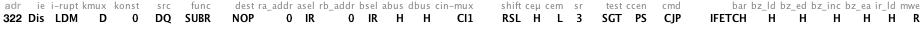
\includegraphics[width=18cm]{cmp_3.png}} \\[0.3cm]
    \hline
   Der Wert, der auf dem Datenbus liegt (entspricht \emph{[ra]}), wird vom Wert des im \emph{Q} zwischengespeicherten Registers \emph{rb} substrahiert und die Maschinenstatusregister-Flags werden entsprechend gesetzt. Das Ergebnis wird verworfen.\\
    \hline
  \end{tabular}
\end{center}

\vspace{0.5cm}

\begin{center}
\rowcolors{1}{lightgray}{white}
\footnotesize
  \begin{tabular}{|p{18cm}|}
  	\hline
    81: jmpz\_imm \\
    \hline
    \raisebox{-0.4cm}{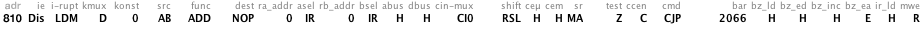
\includegraphics[width=18cm]{jmpz_1.png}} \\[0.3cm]
    \hline
   Der Inhalt des Befehlszählers wird auf den Addressbus geleget und das MWE-Flag wird auf R gesetzt. Falls das Z-Flag des Maschinenstatusregisters gesetzt ist, trifft die Sprungbedingung ein und es wird zur letzten Instruktion des Befehls gesprungen.\\
    \hline

    \raisebox{-0.4cm}{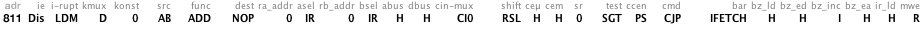
\includegraphics[width=18cm]{jmpz_2.png}} \\[0.3cm]
    \hline
   Die Bedingung ist nicht eingetroffen. Der Befehlszähler wird inkrementiert, um den Immidiate-Wert zu überspringen.\\
    \hline
    
    \raisebox{-0.4cm}{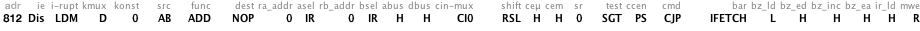
\includegraphics[width=18cm]{jmpz_3.png}} \\[0.3cm]
    \hline
   Die Bedingung ist eingetroffen - führe den Sprung zu \emph{imm} aus. Dem Befehlszähler wird der Wert des D-Eingangs (entspricht \emph{imm}) zugewiesen. Der Befehlszähler wird inkrementiert, um den Immidiatewert zu überspringen.\\
    \hline
    
  \end{tabular}
\end{center}

\vspace{0.5cm}

\begin{center}
\rowcolors{1}{lightgray}{white}
\footnotesize
  \begin{tabular}{|p{18cm}|}
  	\hline
    B0: jmp\_imm \\
    \hline
    \raisebox{-0.4cm}{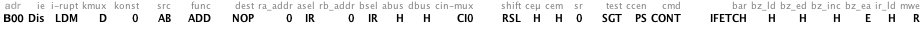
\includegraphics[width=18cm]{jmp_1.png}} \\[0.3cm]
    \hline
   Der Inhlalt des Befehlszählers wird auf den Addressbus geleget und das MWE-Flag auf R gesetzt.\\
    \hline
    
    \raisebox{-0.4cm}{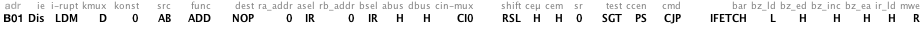
\includegraphics[width=18cm]{jmp_2.png}} \\[0.3cm]
    \hline
   Dem Befehlszähler wird der Wert des D-Eingangs (entspricht \emph{imm}) zugewiesen.\\
    \hline
    
  \end{tabular}
\end{center}

\subsection{Anmerkungen}
\begin{enumerate}
\item Keine der Implementierungen überprüft, ob das aktuelle Zeichen tatsächlich ein Unicode-Zeichen ist. Es wird lediglich überprüft, ob es sich um das Nullzeichen (0x0000) handelt.
\item Register \emph{r1} darf in der Mikroprogrammimplementierung nicht als Quellopearand (RA) übergeben werden, da es als Ergebnis-Register eingesetzt wird.
\end{enumerate}



\subsection{Effizienzvergleich}

An der Anzahl der nötigen IFETCH-Operationen beider Implementierungen ist leicht zu erkennen, dass das Mikroprogramm deutlich effizienter arbeitet als das Maschinenprogramm. Im Folgenden wird die Messung einer Zeichenkette der Länge n betrachtet. Je länger die Zeichenkette ist, desto größer ist der Effizienzunterschied, da hier die Anzahl der ausgeführten IFETCH-Operationen entsprechend steigt.

\begin{itemize}
\item \emph{Maschinenprogramm}:\newline 2 (Initialisierung) + 4n (Schleife) + 2 (Nullzeichen) + 1 (Subtraktion) =\newline 4n + 5 IFETCH-Operationen = (4n + 5) * 3 Takte =\newline {\bf 12n + 15 Takte allein für IFETCH-Operationen}
\item \emph{Mikroprogramm}:\newline 3 (IFETCH) + 4n (Schleife) + 3 (Nullzeichen) + 1 (Subtraktion) =\newline {\bf 4n + 8 Takte insgesamt}
\end{itemize}

\newpage

\section{Tests}

Die Programme mit den Testfällen wurden in separaten Dateien mit folgendem Format gespeichert: \emph{strlen\_ProgrammName\_TestCaseName\_(Assertion=Value).mpr}. Die Tests für das Mikroprogramm wurden in einer gesonderten Datei gespeichert, da hier die Möglichkeit besteht, für jeden Testfall einen separaten Aufruf des Mikroprogramms auszuführen. Beide Implementierungen wurden mit folgenden Belegungen getestet:

\begin{enumerate}
\item empty\_string: Dem Programm wird die Adresse einer Zelle mit dem Nullzeichen (0x0000) übergeben. Das Programm sollte 0 ausgeben.
\item normal\_string: Dem Programm wird die Anfangsadresse einer Zeichenkette mit 9 Zeichen übergeben. Das Programm sollte 9 ausgeben
\item long\_string: Dem Programm wird die Anfangsadresse einer Zeichenkette mit 32 bzw. 22 (Mikro) Zeichen übergeben. Das Programm sollte 32 bzw. 22 ausgeben.
\item two\_strings: Zwei Zeichenketten wurden direkt nacheinander im Speicher abgelegt. Dem Programm wird die Addresse der ersten Zeichenkette übergeben. Das Programm sollte die Länge der ersten Zeichenkette (5) ausgeben.
\end{enumerate}

\section{Alternative Lösungsansätze}
\begin{enumerate}
\item Die beiden Programme könnten mithilfe eines Zählers, der die Anzahl der überprüften Zeichen speichert, implementiert werden. Diese Lösung würde jedoch einen zusätzlichen Befehl (Inkrementieren des Zählers) innerhalb der \emph{while}-Schleife benötigen, wodurch sich die Effizienz verringern würde.
\item Statt im Mikroprogramm das Ergebnis fix in \emph{r1} zu speichern, wäre es besser ein gewünschtes Zielregister über den Zieloperanden (RB) zu übergeben.
\end{enumerate}

\end{document}